\documentclass[twoside,11pt]{article}

\usepackage{blindtext}
\usepackage{tabularx} %
\usepackage[table]{xcolor} %
\usepackage{url}
\usepackage{jmlr2e}
\usepackage{graphicx} %
\usepackage{booktabs} %
\usepackage{multirow} %
\usepackage{amsmath} %
\newcommand{\dataset}{{\cal D}}
\newcommand{\fracpartial}[2]{\frac{\partial #1}{\partial  #2}}
\usepackage{lastpage}
\jmlrheading{23}{2022}{1-\pageref{LastPage}}{1/21; Revised 5/22}{9/22}{21-0000}{Professor Cline}
\ShortHeadings{pyFAST: A Modular PyTorch Framework for Time Series Modeling}{pyFAST: A Modular PyTorch Framework for Time Series Modeling}
\firstpageno{1}

\usepackage{enumerate}

\begin{document}

\title{pyFAST: A Modular PyTorch Framework for Multi-source and Sparse Time Series Modeling and Benchmarking}


\author{
    \name Zhijin Wang, Senzhen Wu \email zhijinecnu@gmail.com,~szwbyte@gmail.com \\
    \addr College of Computer Engineering\\
    Jimei University\\
    Xiamen 361021, China
    \AND
    \name Xiufeng Liu \email xiuli@dtu.dk \\
    \addr Department of Technology, Management and Economics\\
    Technical University of Denmark\\
    Lyngby 2800, Denmark
}

\editor{My editor}

\maketitle

\begin{abstract}
Modern time series analysis demands flexible, efficient, and extensible software; yet existing Python libraries often fall short, lacking modularity and support for cutting-edge models, especially for tasks like univariate forecasting and sparse data handling. To bridge this gap, we introduce \texttt{pyFAST}, a novel, research-driven Python framework that redefines modularity and efficiency in time series analysis. \texttt{pyFAST} pioneers the integration of Large Language Model (LLM) principles to handle multi-source time series data without requiring strict temporal alignment, a unique capability for flexible data integration. It offers native support for sparse data and provides specialized sparse metrics and loss functions, alongside a comprehensive suite of state-of-the-art models, including Transformers and Graph Neural Networks. Its unique modular architecture empowers users to seamlessly customize and extend the library, fostering rapid experimentation and methodological innovation. Benchmarking demonstrates \texttt{pyFAST}'s superior computational efficiency and competitive accuracy against leading libraries. \texttt{pyFAST} is publicly available at \href{https://github.com/freepose/pyFAST}{\textit{https://github.com/freepose/pyFAST}}, implemented in PyTorch and released under the MIT license, with comprehensive documentation and examples, aiming to catalyze community contributions and accelerate advancements in time series research and applications.
\end{abstract}

\section{Introduction}
Time series analysis is indispensable across diverse domains, from financial forecasting and healthcare monitoring to environmental science and industrial predictive maintenance. Despite the availability of powerful libraries such as TensorFlow Time Series \citep{abadi2016tensorflow}, GluonTS \citep{alexandrov2020gluonts}, and PyTorch Forecasting \citep{paszke2019pytorch}, significant challenges remain in modularity, flexibility, and support for cutting-edge research. Existing tools often specialize in specific model families or lack the architectural openness to incorporate novel algorithms and adapt to diverse application needs, thereby hindering rapid experimentation and innovation. Specifically, many libraries lack native support for sparse time series data and the flexibility to easily implement and test novel model architectures, such as recent advancements in applying Large Language Models to time series forecasting.  Furthermore, the ability to effectively fuse exogenous data and handle multi-source time series without strict temporal alignment remains a significant unmet need. To overcome these limitations, we present \texttt{pyFAST}, a novel research-driven Python framework for modular and efficient time series analysis.  \texttt{pyFAST} uniquely integrates LLM-inspired architectures for alignment-free multi-source time series processing, native sparse data support with specialized metrics, and comprehensive functionalities for exogenous data fusion and sequence learning, including protein prediction. This comprehensive and adaptable toolkit empowers researchers and practitioners to seamlessly incorporate cutting-edge models and custom modifications for diverse time series tasks across research and real-world applications, such as healthcare and energy forecasting.


\section{Software Overview}
\begin{figure}[htbp]
    \centering
    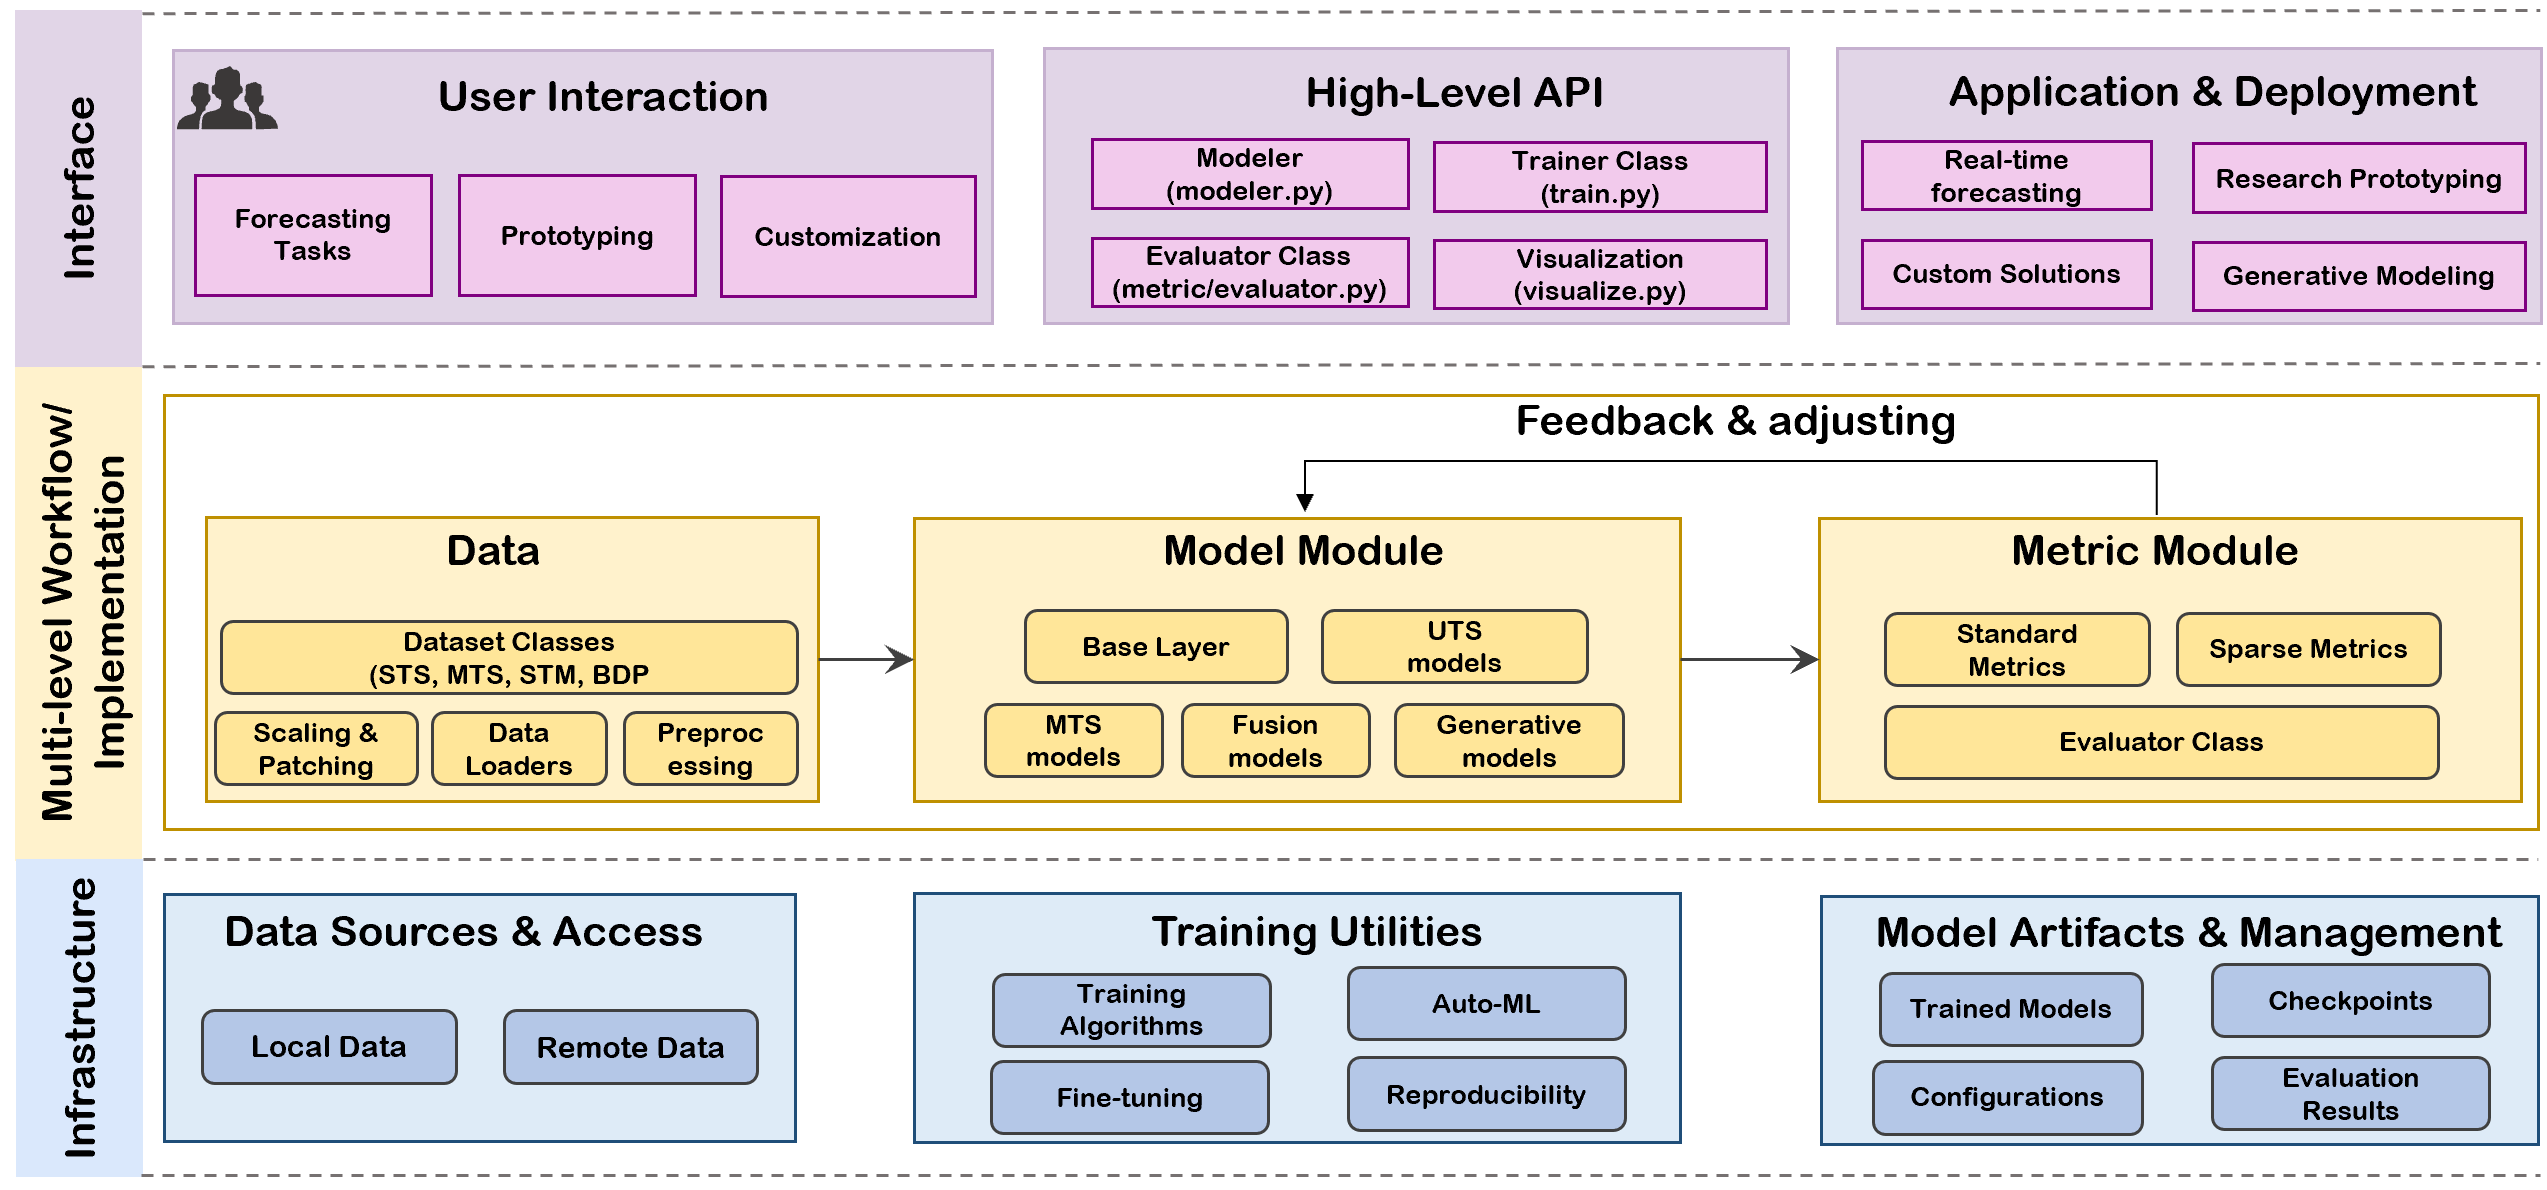
\includegraphics[width=0.4\textwidth]{figures/software_overview.png}
    \caption{Software Overview of pyFAST Library}
    \label{fig:software_overview}
\end{figure}
\texttt{pyFAST} is architected around modularity, with each component engineered to address a specific facet of time series analysis. This modular design philosophy enhances flexibility, maintainability, and extensibility, allowing users to tailor the library to diverse analytical tasks. The library’s core functionalities are organized into five modules, each designed with specific capabilities. The \texttt{data} module handles data loading and preprocessing with dataset classes for STS, MTM, BDP, and STM, and scaling methods. Notably, the \texttt{data} module is designed to efficiently handle sparse data and facilitate the integration of multi-source datasets, even those lacking temporal alignment. This is achieved through specialized data loaders and preprocessing techniques that accommodate varying data granularities and sparsity patterns. It enables flexible data pipeline construction. The \texttt{model} module hosts a diverse collection of time series models, including classical, deep learning (CNNs, RNNs, Transformers), and GNN-based architectures for both UTS and MTS data. For sequence learning tasks, \texttt{pyFAST} provides support for batch-wise dynamic padding, enabling efficient processing of variable-length sequences, crucial for applications such as protein prediction. The \texttt{base} submodule provides fundamental building blocks for custom model creation. The \texttt{train} module provides the \texttt{Trainer} class, streamlining model training with functionalities for validation, early stopping, checkpointing, and support for various optimization and learning rate scheduling techniques. The \texttt{metric} module offers a comprehensive suite of evaluation metrics for time series tasks, including specialized sparse metrics tailored for masked and sparse data, such as Sparse Mean Squared Error and Sparse Mean Absolute Error. The \texttt{Evaluator} class simplifies results reporting. The \texttt{visualize} module aids model analysis and interpretation through time series data and prediction visualizations. \texttt{pyFAST}'s modular architecture empowers researchers and practitioners to extend and customize and combine modules for reproducible state-of-the-art models.

\section{Comparison with Related Work}
The landscape of time series modeling libraries and frameworks is rich and diverse, with several excellent tools available to researchers and practitioners. TensorFlow Time Series \citep{abadi2016tensorflow} provides a comprehensive and mature toolkit within the TensorFlow ecosystem, with a strong focus on forecasting and anomaly detection. GluonTS \citep{alexandrov2020gluonts}, developed by Amazon, is a widely adopted library renowned for its extensive suite of probabilistic forecasting models and specialized tools for handling probabilistic time series prediction. PyTorch Forecasting \citep{paszke2019pytorch} offers a collection of time series-specific layers, models, and training utilities within the PyTorch framework, emphasizing explainable and interpretable forecasting methodologies. `sktime' \citep{loning2019sktime} stands out as a comprehensive Python toolbox encompassing a wide range of time series analysis tasks, including classical models, machine learning models, and sophisticated evaluation tools, with a strong emphasis on seamless integration with the scikit-learn ecosystem. `tslearn' \citep{tavenard2020tslearn} specializes in time series-specific machine learning algorithms, offering tools for time series clustering, classification, representation learning, and related tasks, and also incorporates shapelet learning methods. StatsForecast \citep{garza2022statsforecast} and NeuralForecast \citep{olivares2022library_neuralforecast} are highly optimized libraries specifically engineered for fast and scalable forecasting, providing efficient implementations of both statistical and neural forecasting models, respectively, with a focus on computational performance. Time-Series-Library (TSLib) \citep{wu2023timesnet} from Tsinghua University offers a collection of time series algorithms and models, emphasizing efficiency and reproducibility. While TSLib provides a solid foundation for time series research, it primarily focuses on standard time series tasks and lacks native support for advanced features such as multi-source data handling without alignment and specialized sparse data functionalities.

\begin{table*}[t!]
    \centering
    \caption{Comparison of \texttt{pyFAST} with Related Time Series Libraries}
    \label{tab:library_comparison}
    \rowcolors{2}{white}{gray!15} %
    {\scriptsize
    \begin{tabularx}{\textwidth}{@{}p{1.6cm}p{3cm}p{2.1cm}p{2.1cm}p{2.1cm}p{2.1cm}@{}}
    \toprule
    \textbf{Feature} & \textbf{\texttt{pyFAST}} & \textbf{GluonTS} & \textbf{PyTorch Forecasting} & \textbf{sktime} & \textbf{TSLib} \\
    \midrule
    Modularity & \textbf{High} (Component-based, highly customizable) & Medium (Model zoo, some customization) & Medium (Layer-based, some customization) & High (Class-based, extensible framework) & Medium (Modular design) \\
    Extensibility & \textbf{High} (Easy to add custom models/components) & Medium (Adding new models requires effort) & Medium (Custom layers supported) & High (Extensible class hierarchy, well-defined interfaces) & Medium (Extensible, but might require deeper code modification) \\
    Model Breadth (DL \& Classical) & \textbf{Extensive} (Deep learning \& classical statistical models) & Broad (Strong DL, limited classical) & Broad (Classical ML and deep learning) & Broad (Classical statistical \& ML models) & Broad (Focus on deep learning, but includes classical) \\
    Transformer Models & \textbf{Extensive} (PatchTST, Informer, Autoformer, diverse variants) & Limited (Basic Transformer encoder-decoder) & Yes (Time series Transformer layers) & Limited (No dedicated Transformer models) & Yes (Transformer models included) \\
    LLM-Inspired Models \& Multi-source Support & \textbf{Yes} (Transformer-based LLM adaptations, \textbf{native multi-source support without alignment}) & No & No & No & No \\
    Sparse Data Support & \textbf{Yes} (\textbf{native sparse data support, sparse metrics and losses}) & No & No & No & No \\
    Exogenous Data Fusion & \textbf{Yes} (\textbf{flexible exogenous data integration}) & Yes & Yes & Yes & Yes \\
    Sequence Learning Focus & \textbf{Yes} (\textbf{batch-wise dynamic padding for variable-length sequences}) & Yes & Yes & Yes & Yes \\
    Imputation & \textbf{Yes} (Dedicated imputation models/methods) & Yes (Probabilistic models can be adapted for imputation) & Limited (Imputation not a primary focus) & Yes (Comprehensive toolbox includes imputation methods) & Limited (Imputation not explicitly highlighted) \\
    Benchmarking Suite & \textbf{Yes} (Standardized benchmarking framework) & Limited (Basic benchmarks) & No & Yes (Comprehensive evaluation framework) & Yes (Benchmarking scripts provided) \\
    Focus & \textbf{Research \& Prototyping} (Flexibility and customization) & \textbf{Probabilistic Forecasting} (Scalability and uncertainty estimation) & \textbf{Explainability} (Interpretability and time series-specific layers) & \textbf{General Time Series Analysis} (Broad toolbox for diverse tasks) & \textbf{Efficiency \& Reproducibility} (Emphasis on performance and code clarity) \\
    \bottomrule
    \end{tabularx}
    }
\end{table*}
Table \ref{tab:library_comparison} provides a detailed comparative analysis of \texttt{pyFAST} against these key related libraries, highlighting their respective strengths and weaknesses across a range of features relevant to time series research and application development. Table \ref{tab:library_comparison} shows \texttt{pyFAST}'s unique combination of LLM-inspired multi-source handling, sparse data support, and modularity, setting it apart from specialized or inflexible libraries. Compared to TSLib, \texttt{pyFAST} excels in advanced research capabilities with pioneering LLM and sparse data features, while both offer efficiency and benchmarking. \texttt{pyFAST} prioritizes cutting-edge research and rapid prototyping, offering researchers a highly flexible and customizable platform to explore time series modeling frontiers. Its standardized benchmarking suite promotes reproducible research and method comparisons. The modular architecture and comprehensive features make \texttt{pyFAST} ideal for researchers requiring fine-grained control over model design, training, and evaluation, aiming to advance time series modeling research.

\section{Conclusion}
In conclusion, \texttt{pyFAST} is a novel, modular, efficient, and comprehensive Python library designed to empower time series researchers and practitioners.  Its key strengths include unique multi-source and sparse data handling, research-driven flexibility, and a diverse model library with LLM-inspired architectures. Benchmarking validates its practical utility and competitive performance. We believe \texttt{pyFAST} offers a valuable, high-performance, and adaptable platform for driving future innovations across time series research and applications. \texttt{pyFAST} is publicly available at \href{https://github.com/freepose/pyFAST}{GitHub}, accompanied by extensive resources to support and expand its community of users and contributors.
\bibliography{refs}
\end{document}